\documentclass[../documentation.tex]{subfiles}
 
\begin{document}

\section{Projekt részletes leírása} \label{sec:projectdescription}
A projekt célja egy olyan robot bemutató hardveres és szoftveres kidolgozása, amely képes egy emberrel (továbbfejlesztés után akár egy másik robottal) lejátszani egy sakkjátszmát. A bemutató az ember-robot kollaboráció szemléltetésére szolgál. Fontos szempont az interakció biztonságos megvalósítása mind az emberre, mind a környező tárgyakra tekintettel.

A projekthez egy KUKA gyártmányú LBR iiwa 7 típusú robotkar került felhasználásra (\ref{fig:iiwa} ábra).\footnotetext{A kép forrása: \url{https://www.businesswire.com/news/home/20150320005018/en/KUKA-Robotics-Corporation-debuts-LBR-iiwa-North}, 2018.11.25.}

\begin{figure}[h]
\centering
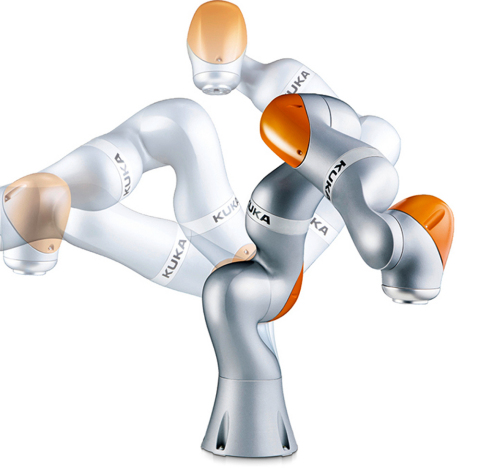
\includegraphics[scale=0.50]{iiwa}
\caption{A projekthez használt robotkar\protect\footnotemark}
\label{fig:iiwa}
\end{figure}

A megvalósításhoz a következő problémák megoldására van szükség:
\begin{enumerate}
	\item szükséges biztonsági funkciók beüzemelése,
	\item a bábuk helyzetének felismerése az egyes lépések előtt és után,
	\item a kamera kiválasztása és robotvezérlőhöz illesztése (a bábuk helyzetének felismeréséhez),
	\item a bábuk megfogása és mozgatása (ide tartozik a kalibráció, a referenciafelvétel és a megfogó vezérlése is),
	\item kiválasztott sakkalgoritmus beágyazása a programba,
	\item a sakkbábúk és a tábla megtervezése és megvalósítása,
	\item jelzés a robotkar számára, ha lépés történt.
\end{enumerate}
A felsorolt pontok a projekt során a következőképpen kerültek kidolgozásra:
\begin{itemize}
	\item A bábuk helyzetének detektálása a projekt során zöld szín szűrő képfeldogozó eljáráson alapul (a bábuk tetején zöld színű lap található). A kamera a roboton kerül rögzítésre.
	\item A bábuk mozgatása egy elektromosan vezérelt, párhuzamos megfogó (\angol{gripper}) segítségével történik.
	\item Ahhoz hogy a bábuk megfogása egyszerű legyen, azonos magasságú és azonos módszerrel megfogható bábuk készültek.
	\item A biztonsági funkciók főként az tengelyekben ébredő plusz nyomatékok monitorozására épül.
	\item A tábla és a robotkar, illetve a megfogó (egy jól definiált pontja) és a robotkar relatív helyzetének kalibrálására a robotvezérlő szoftverben elérhető alapfunkciók kerültek felhasználásra.
	\item A sakklépés megtörténtét a robotvezérlőhöz tartozó smartPAD-en lehet jelezni.
	\item A képek fogadása, feldolgozása és a sakkalgoritmus futtatása is mind a robotvezérlőn történik.
	\item Mivel a robotvezérlőn Java alapú környezet fut magas szinten, így a képfeldolgozó és a sakkprogram is ebben lett implementálva.
\end{itemize}

A projekt főként 4 modulból áll: képkészítés, képfeldolgozás, sakkprogram és robotvezérlés. Ezek kidolgozásánál fontos szempont a modulok közötti kapcsolat is. A projekt folyamatábráját \aref{fig:flowchart} ábra mutatja. A most következő fejezetek a folyamatábra elemeit igyekszenek bemutatni.

\begin{figure}[h]
\centering
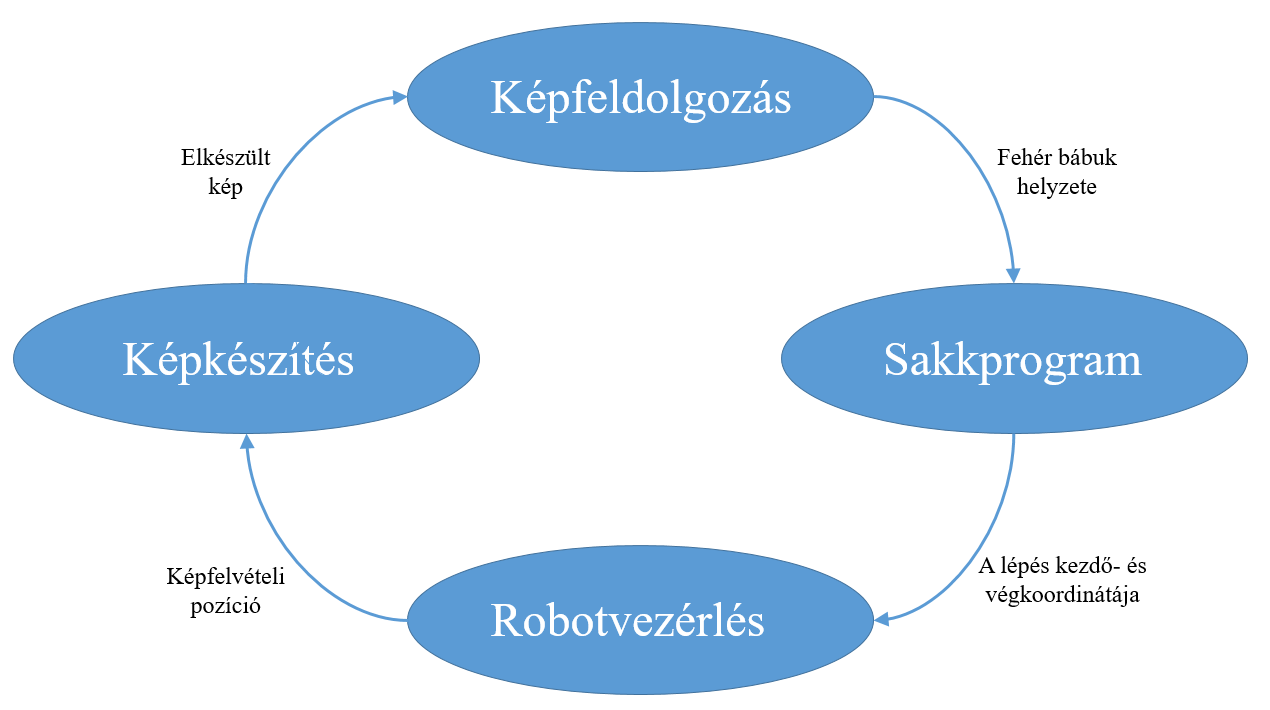
\includegraphics[scale=0.45]{flowchart}
\caption{A fő modulok és az azok közötti kapcsolat}
\label{fig:flowchart}
\end{figure}

\end{document}